\hypertarget{_lgm___lstar_info_8h}{
\section{/home/mgh/LanlGeoMag/libLanlGeoMag/Lgm/Lgm\_\-LstarInfo.h File Reference}
\label{_lgm___lstar_info_8h}\index{/home/mgh/LanlGeoMag/libLanlGeoMag/Lgm/Lgm\_\-LstarInfo.h@{/home/mgh/LanlGeoMag/libLanlGeoMag/Lgm/Lgm\_\-LstarInfo.h}}
}
{\tt \#include $<$math.h$>$}\par
{\tt \#include \char`\"{}Lgm\_\-QuadPack.h\char`\"{}}\par
{\tt \#include \char`\"{}Lgm\_\-MagModelInfo.h\char`\"{}}\par
{\tt \#include $<$gsl/gsl\_\-errno.h$>$}\par
{\tt \#include $<$gsl/gsl\_\-spline.h$>$}\par


Include dependency graph for Lgm\_\-LstarInfo.h:\nopagebreak
\begin{figure}[H]
\begin{center}
\leavevmode
\includegraphics[width=295pt]{_lgm___lstar_info_8h__incl}
\end{center}
\end{figure}


This graph shows which files directly or indirectly include this file:\nopagebreak
\begin{figure}[H]
\begin{center}
\leavevmode
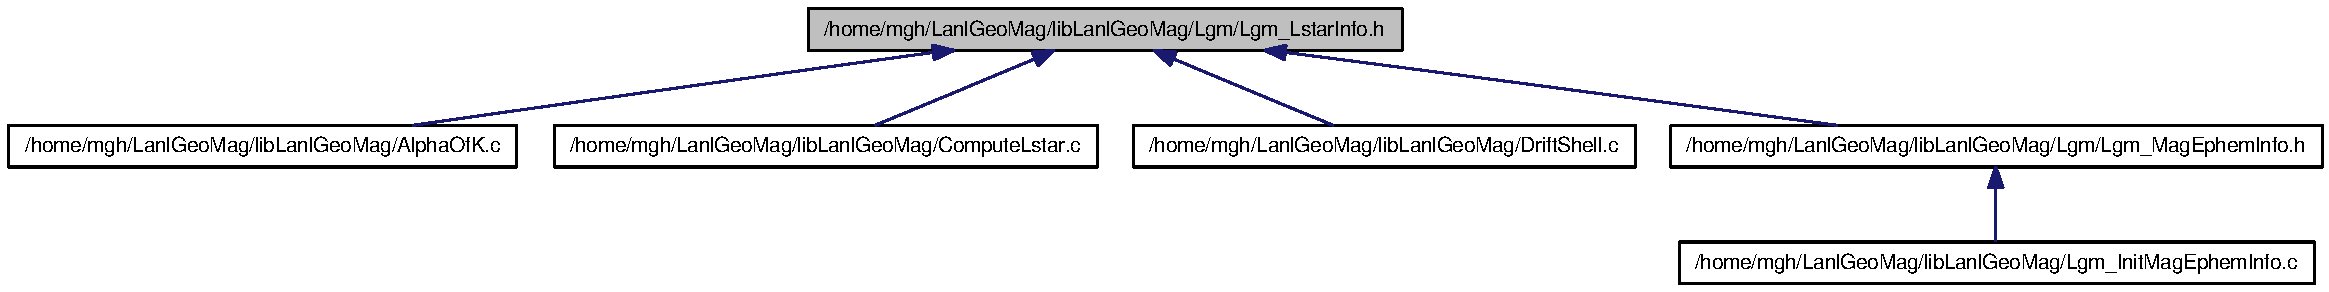
\includegraphics[width=420pt]{_lgm___lstar_info_8h__dep__incl}
\end{center}
\end{figure}
\subsection*{Data Structures}
\begin{CompactItemize}
\item 
struct \hyperlink{struct_lgm___lstar_info}{Lgm\_\-LstarInfo}
\end{CompactItemize}
\subsection*{Defines}
\begin{CompactItemize}
\item 
\#define \hyperlink{_lgm___lstar_info_8h_1f6f907234204d7207579a18fb0847a4}{ELECTRON\_\-MASS}~(9.10938188e-31)
\item 
\#define \hyperlink{_lgm___lstar_info_8h_e72e484b3bba78248e0f70f47d11cb43}{AMU}~(1.660538e-27)
\item 
\#define \hyperlink{_lgm___lstar_info_8h_b8cacd34cfff7982e36652a0330d8d83}{PROTON\_\-MASS}~(1.00794$\ast$AMU)
\item 
\#define \hyperlink{_lgm___lstar_info_8h_d6cde5694a5a86aafb92eecd7cf439be}{OXYGEN\_\-MASS}~(15.9994$\ast$AMU)
\item 
\#define \hyperlink{_lgm___lstar_info_8h_0600e3f227b6e9a3ae26f4d6e2a0581e}{RE}~(6378.135e3)
\item 
\#define \hyperlink{_lgm___lstar_info_8h_78d126676907aa89a0adbfbef8282585}{CC}~(2.99792458e8)
\item 
\#define \hyperlink{_lgm___lstar_info_8h_40069882b1f09d9463acc3acd7b67708}{EE}~(1.6022e-19)
\end{CompactItemize}
\subsection*{Functions}
\begin{CompactItemize}
\item 
void \hyperlink{_lgm___lstar_info_8h_08977c566a558f0198da8d01ea0677f1}{SetLstarTolerances} (int Quality, \hyperlink{struct_lgm___lstar_info}{Lgm\_\-LstarInfo} $\ast$LstarInfo)
\item 
\hyperlink{struct_lgm___lstar_info}{Lgm\_\-LstarInfo} $\ast$ \hyperlink{_lgm___lstar_info_8h_d7d999fbe5d3b065fe808bb3e7ceab0b}{InitLstarInfo} (int VerbosityLevel)
\item 
void \hyperlink{_lgm___lstar_info_8h_edbca525fb67c0d6cde4b890ff37c1a3}{FreeLstarInfo} (\hyperlink{struct_lgm___lstar_info}{Lgm\_\-LstarInfo} $\ast$LstarInfo)
\item 
\hyperlink{struct_lgm___lstar_info}{Lgm\_\-LstarInfo} $\ast$ \hyperlink{_lgm___lstar_info_8h_84a1ec912704573c21c1e506b72d6f01}{Lgm\_\-CopyLstarInfo} (\hyperlink{struct_lgm___lstar_info}{Lgm\_\-LstarInfo} $\ast$s)
\item 
double \hyperlink{_lgm___lstar_info_8h_a9a43909d59850c622768267ce73421c}{AlphaOfK} (double K, \hyperlink{struct_lgm___lstar_info}{Lgm\_\-LstarInfo} $\ast$LstarInfo)
\item 
int \hyperlink{_lgm___lstar_info_8h_fa76ff04b6e63787c11731095a1aa6fb}{Grad\_\-I} (\hyperlink{struct_lgm___vector}{Lgm\_\-Vector} $\ast$vin, \hyperlink{struct_lgm___vector}{Lgm\_\-Vector} $\ast$GradI, \hyperlink{struct_lgm___lstar_info}{Lgm\_\-LstarInfo} $\ast$LstarInfo)
\item 
int \hyperlink{_lgm___lstar_info_8h_c2ed60f1d1f9d07a4715095c94e131fe}{ComputeVcg} (\hyperlink{struct_lgm___vector}{Lgm\_\-Vector} $\ast$vin, \hyperlink{struct_lgm___vector}{Lgm\_\-Vector} $\ast$Vcg, \hyperlink{struct_lgm___lstar_info}{Lgm\_\-LstarInfo} $\ast$LstarInfo)
\item 
int \hyperlink{_lgm___lstar_info_8h_15d887d6b99cb83ce58b5a04a171ec67}{FindBmRadius} (double Bm, double MLT, double mlat, double $\ast$r, double tol, \hyperlink{struct_lgm___lstar_info}{Lgm\_\-LstarInfo} $\ast$LstarInfo)
\item 
int \hyperlink{_lgm___lstar_info_8h_e79603e88bcb7860ca33e8fe4fbdf37f}{FindShellLine} (double I0, double $\ast$Ifound, double Bm, double MLT, double $\ast$mlat, double $\ast$rad, double mlat0, double mlat1, \hyperlink{struct_lgm___lstar_info}{Lgm\_\-LstarInfo} $\ast$LstarInfo)
\item 
void \hyperlink{_lgm___lstar_info_8h_e2e73ba3832c389e53954019ceb47ded}{spline} (double $\ast$x, double $\ast$y, int n, double yp1, double ypn, double $\ast$y2)
\item 
void \hyperlink{_lgm___lstar_info_8h_219484a4d3318d5361a52365d97cddc3}{splint} (double $\ast$xa, double $\ast$ya, double $\ast$y2a, int n, double x, double $\ast$y)
\item 
void \hyperlink{_lgm___lstar_info_8h_e2628883d2b8f49b8df3690a121f1e40}{quicksort} (unsigned long n, double $\ast$arr)
\item 
void \hyperlink{_lgm___lstar_info_8h_3801a78bfafe0c674baf406ff2531f3e}{quicksort2} (unsigned long n, double $\ast$arr, double $\ast$brr)
\item 
\hyperlink{struct_lgm___mag_model_info}{Lgm\_\-MagModelInfo} $\ast$ \hyperlink{_lgm___lstar_info_8h_0d0473dc2b48c646fb6cf5297ba74636}{init\_\-info} ()
\item 
void \hyperlink{_lgm___lstar_info_8h_68ec464c1b33f0b437d856629f0dd901}{NewTimeLstarInfo} (long int Date, double UT, double PitchAngle, int($\ast$Mag)(\hyperlink{struct_lgm___vector}{Lgm\_\-Vector} $\ast$, \hyperlink{struct_lgm___vector}{Lgm\_\-Vector} $\ast$, \hyperlink{struct_lgm___mag_model_info}{Lgm\_\-MagModelInfo} $\ast$), \hyperlink{struct_lgm___lstar_info}{Lgm\_\-LstarInfo} $\ast$LstarInfo)
\item 
int \hyperlink{_lgm___lstar_info_8h_957a4d60eb4025656b3c2557b402523e}{Lstar} (\hyperlink{struct_lgm___vector}{Lgm\_\-Vector} $\ast$vin, \hyperlink{struct_lgm___lstar_info}{Lgm\_\-LstarInfo} $\ast$LstarInfo)
\item 
double \hyperlink{_lgm___lstar_info_8h_871565dbd20b1df061fb2e706bd724db}{MagFlux} (\hyperlink{struct_lgm___lstar_info}{Lgm\_\-LstarInfo} $\ast$LstarInfo)
\item 
double \hyperlink{_lgm___lstar_info_8h_7da6f58b128b4aef809400ada95767d4}{MagFlux2} (\hyperlink{struct_lgm___lstar_info}{Lgm\_\-LstarInfo} $\ast$LstarInfo)
\item 
double \hyperlink{_lgm___lstar_info_8h_5f75b0909329fb6260c63bc551c29acb}{MagFluxIntegrand} (double Phi, \hyperlink{_lgm___quad_pack_8h_01be5a7db8d2fc2ba26ce793d73b6472}{\_\-qpInfo} $\ast$qpInfo)
\item 
double \hyperlink{_lgm___lstar_info_8h_0f767b7206b1928b2f36fa7c5a26ca33}{MagFluxIntegrand2} (double Phi, \hyperlink{_lgm___quad_pack_8h_01be5a7db8d2fc2ba26ce793d73b6472}{\_\-qpInfo} $\ast$qpInfo)
\item 
double \hyperlink{_lgm___lstar_info_8h_fb4cfc3e9728d5ec4867d39f1384dc38}{LambdaIntegrand} (double Lambda, \hyperlink{_lgm___quad_pack_8h_01be5a7db8d2fc2ba26ce793d73b6472}{\_\-qpInfo} $\ast$qpInfo)
\item 
double \hyperlink{_lgm___lstar_info_8h_593bd0ac5cd8b137cbc401b58219df31}{LambdaIntegral} (\hyperlink{struct_lgm___lstar_info}{Lgm\_\-LstarInfo} $\ast$LstarInfo)
\item 
double \hyperlink{_lgm___lstar_info_8h_48c5ace9102643dda45f657ddb8aac3c}{AngVelInv} (double Phi)
\end{CompactItemize}


\subsection{Define Documentation}
\hypertarget{_lgm___lstar_info_8h_1f6f907234204d7207579a18fb0847a4}{
\index{Lgm\_\-LstarInfo.h@{Lgm\_\-LstarInfo.h}!ELECTRON\_\-MASS@{ELECTRON\_\-MASS}}
\index{ELECTRON\_\-MASS@{ELECTRON\_\-MASS}!Lgm_LstarInfo.h@{Lgm\_\-LstarInfo.h}}
\subsubsection[{ELECTRON\_\-MASS}]{\setlength{\rightskip}{0pt plus 5cm}\#define ELECTRON\_\-MASS~(9.10938188e-31)}}
\label{_lgm___lstar_info_8h_1f6f907234204d7207579a18fb0847a4}




Definition at line 10 of file Lgm\_\-LstarInfo.h.\hypertarget{_lgm___lstar_info_8h_e72e484b3bba78248e0f70f47d11cb43}{
\index{Lgm\_\-LstarInfo.h@{Lgm\_\-LstarInfo.h}!AMU@{AMU}}
\index{AMU@{AMU}!Lgm_LstarInfo.h@{Lgm\_\-LstarInfo.h}}
\subsubsection[{AMU}]{\setlength{\rightskip}{0pt plus 5cm}\#define AMU~(1.660538e-27)}}
\label{_lgm___lstar_info_8h_e72e484b3bba78248e0f70f47d11cb43}




Definition at line 11 of file Lgm\_\-LstarInfo.h.\hypertarget{_lgm___lstar_info_8h_b8cacd34cfff7982e36652a0330d8d83}{
\index{Lgm\_\-LstarInfo.h@{Lgm\_\-LstarInfo.h}!PROTON\_\-MASS@{PROTON\_\-MASS}}
\index{PROTON\_\-MASS@{PROTON\_\-MASS}!Lgm_LstarInfo.h@{Lgm\_\-LstarInfo.h}}
\subsubsection[{PROTON\_\-MASS}]{\setlength{\rightskip}{0pt plus 5cm}\#define PROTON\_\-MASS~(1.00794$\ast$AMU)}}
\label{_lgm___lstar_info_8h_b8cacd34cfff7982e36652a0330d8d83}




Definition at line 12 of file Lgm\_\-LstarInfo.h.\hypertarget{_lgm___lstar_info_8h_d6cde5694a5a86aafb92eecd7cf439be}{
\index{Lgm\_\-LstarInfo.h@{Lgm\_\-LstarInfo.h}!OXYGEN\_\-MASS@{OXYGEN\_\-MASS}}
\index{OXYGEN\_\-MASS@{OXYGEN\_\-MASS}!Lgm_LstarInfo.h@{Lgm\_\-LstarInfo.h}}
\subsubsection[{OXYGEN\_\-MASS}]{\setlength{\rightskip}{0pt plus 5cm}\#define OXYGEN\_\-MASS~(15.9994$\ast$AMU)}}
\label{_lgm___lstar_info_8h_d6cde5694a5a86aafb92eecd7cf439be}




Definition at line 13 of file Lgm\_\-LstarInfo.h.\hypertarget{_lgm___lstar_info_8h_0600e3f227b6e9a3ae26f4d6e2a0581e}{
\index{Lgm\_\-LstarInfo.h@{Lgm\_\-LstarInfo.h}!RE@{RE}}
\index{RE@{RE}!Lgm_LstarInfo.h@{Lgm\_\-LstarInfo.h}}
\subsubsection[{RE}]{\setlength{\rightskip}{0pt plus 5cm}\#define RE~(6378.135e3)}}
\label{_lgm___lstar_info_8h_0600e3f227b6e9a3ae26f4d6e2a0581e}




Definition at line 14 of file Lgm\_\-LstarInfo.h.\hypertarget{_lgm___lstar_info_8h_78d126676907aa89a0adbfbef8282585}{
\index{Lgm\_\-LstarInfo.h@{Lgm\_\-LstarInfo.h}!CC@{CC}}
\index{CC@{CC}!Lgm_LstarInfo.h@{Lgm\_\-LstarInfo.h}}
\subsubsection[{CC}]{\setlength{\rightskip}{0pt plus 5cm}\#define CC~(2.99792458e8)}}
\label{_lgm___lstar_info_8h_78d126676907aa89a0adbfbef8282585}




Definition at line 15 of file Lgm\_\-LstarInfo.h.\hypertarget{_lgm___lstar_info_8h_40069882b1f09d9463acc3acd7b67708}{
\index{Lgm\_\-LstarInfo.h@{Lgm\_\-LstarInfo.h}!EE@{EE}}
\index{EE@{EE}!Lgm_LstarInfo.h@{Lgm\_\-LstarInfo.h}}
\subsubsection[{EE}]{\setlength{\rightskip}{0pt plus 5cm}\#define EE~(1.6022e-19)}}
\label{_lgm___lstar_info_8h_40069882b1f09d9463acc3acd7b67708}




Definition at line 16 of file Lgm\_\-LstarInfo.h.

\subsection{Function Documentation}
\hypertarget{_lgm___lstar_info_8h_08977c566a558f0198da8d01ea0677f1}{
\index{Lgm\_\-LstarInfo.h@{Lgm\_\-LstarInfo.h}!SetLstarTolerances@{SetLstarTolerances}}
\index{SetLstarTolerances@{SetLstarTolerances}!Lgm_LstarInfo.h@{Lgm\_\-LstarInfo.h}}
\subsubsection[{SetLstarTolerances}]{\setlength{\rightskip}{0pt plus 5cm}void SetLstarTolerances (int {\em Quality}, \/  {\bf Lgm\_\-LstarInfo} $\ast$ {\em LstarInfo})}}
\label{_lgm___lstar_info_8h_08977c566a558f0198da8d01ea0677f1}




Definition at line 21 of file ComputeLstar.c.\hypertarget{_lgm___lstar_info_8h_d7d999fbe5d3b065fe808bb3e7ceab0b}{
\index{Lgm\_\-LstarInfo.h@{Lgm\_\-LstarInfo.h}!InitLstarInfo@{InitLstarInfo}}
\index{InitLstarInfo@{InitLstarInfo}!Lgm_LstarInfo.h@{Lgm\_\-LstarInfo.h}}
\subsubsection[{InitLstarInfo}]{\setlength{\rightskip}{0pt plus 5cm}{\bf Lgm\_\-LstarInfo}$\ast$ InitLstarInfo (int {\em VerbosityLevel})}}
\label{_lgm___lstar_info_8h_d7d999fbe5d3b065fe808bb3e7ceab0b}




Definition at line 189 of file ComputeLstar.c.

Here is the call graph for this function:\nopagebreak
\begin{figure}[H]
\begin{center}
\leavevmode
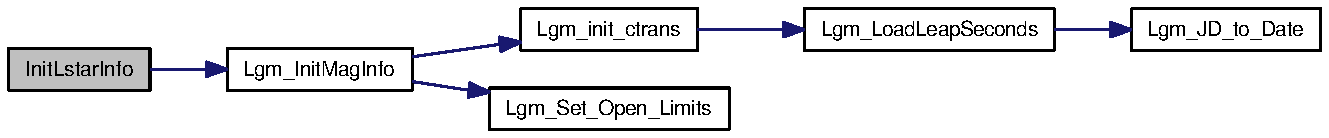
\includegraphics[width=337pt]{_lgm___lstar_info_8h_d7d999fbe5d3b065fe808bb3e7ceab0b_cgraph}
\end{center}
\end{figure}


Here is the caller graph for this function:\nopagebreak
\begin{figure}[H]
\begin{center}
\leavevmode
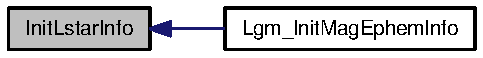
\includegraphics[width=134pt]{_lgm___lstar_info_8h_d7d999fbe5d3b065fe808bb3e7ceab0b_icgraph}
\end{center}
\end{figure}
\hypertarget{_lgm___lstar_info_8h_edbca525fb67c0d6cde4b890ff37c1a3}{
\index{Lgm\_\-LstarInfo.h@{Lgm\_\-LstarInfo.h}!FreeLstarInfo@{FreeLstarInfo}}
\index{FreeLstarInfo@{FreeLstarInfo}!Lgm_LstarInfo.h@{Lgm\_\-LstarInfo.h}}
\subsubsection[{FreeLstarInfo}]{\setlength{\rightskip}{0pt plus 5cm}void FreeLstarInfo ({\bf Lgm\_\-LstarInfo} $\ast$ {\em LstarInfo})}}
\label{_lgm___lstar_info_8h_edbca525fb67c0d6cde4b890ff37c1a3}




Definition at line 221 of file ComputeLstar.c.

Here is the call graph for this function:\nopagebreak
\begin{figure}[H]
\begin{center}
\leavevmode
\includegraphics[width=188pt]{_lgm___lstar_info_8h_edbca525fb67c0d6cde4b890ff37c1a3_cgraph}
\end{center}
\end{figure}


Here is the caller graph for this function:\nopagebreak
\begin{figure}[H]
\begin{center}
\leavevmode
\includegraphics[width=140pt]{_lgm___lstar_info_8h_edbca525fb67c0d6cde4b890ff37c1a3_icgraph}
\end{center}
\end{figure}
\hypertarget{_lgm___lstar_info_8h_84a1ec912704573c21c1e506b72d6f01}{
\index{Lgm\_\-LstarInfo.h@{Lgm\_\-LstarInfo.h}!Lgm\_\-CopyLstarInfo@{Lgm\_\-CopyLstarInfo}}
\index{Lgm\_\-CopyLstarInfo@{Lgm\_\-CopyLstarInfo}!Lgm_LstarInfo.h@{Lgm\_\-LstarInfo.h}}
\subsubsection[{Lgm\_\-CopyLstarInfo}]{\setlength{\rightskip}{0pt plus 5cm}{\bf Lgm\_\-LstarInfo}$\ast$ Lgm\_\-CopyLstarInfo ({\bf Lgm\_\-LstarInfo} $\ast$ {\em s})}}
\label{_lgm___lstar_info_8h_84a1ec912704573c21c1e506b72d6f01}




Definition at line 235 of file ComputeLstar.c.

Here is the call graph for this function:\nopagebreak
\begin{figure}[H]
\begin{center}
\leavevmode
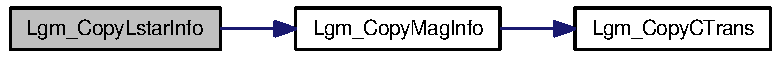
\includegraphics[width=205pt]{_lgm___lstar_info_8h_84a1ec912704573c21c1e506b72d6f01_cgraph}
\end{center}
\end{figure}
\hypertarget{_lgm___lstar_info_8h_a9a43909d59850c622768267ce73421c}{
\index{Lgm\_\-LstarInfo.h@{Lgm\_\-LstarInfo.h}!AlphaOfK@{AlphaOfK}}
\index{AlphaOfK@{AlphaOfK}!Lgm_LstarInfo.h@{Lgm\_\-LstarInfo.h}}
\subsubsection[{AlphaOfK}]{\setlength{\rightskip}{0pt plus 5cm}double AlphaOfK (double {\em K}, \/  {\bf Lgm\_\-LstarInfo} $\ast$ {\em LstarInfo})}}
\label{_lgm___lstar_info_8h_a9a43909d59850c622768267ce73421c}




Definition at line 24 of file AlphaOfK.c.

Here is the call graph for this function:\nopagebreak
\begin{figure}[H]
\begin{center}
\leavevmode
\includegraphics[width=415pt]{_lgm___lstar_info_8h_a9a43909d59850c622768267ce73421c_cgraph}
\end{center}
\end{figure}
\hypertarget{_lgm___lstar_info_8h_fa76ff04b6e63787c11731095a1aa6fb}{
\index{Lgm\_\-LstarInfo.h@{Lgm\_\-LstarInfo.h}!Grad\_\-I@{Grad\_\-I}}
\index{Grad\_\-I@{Grad\_\-I}!Lgm_LstarInfo.h@{Lgm\_\-LstarInfo.h}}
\subsubsection[{Grad\_\-I}]{\setlength{\rightskip}{0pt plus 5cm}int Grad\_\-I ({\bf Lgm\_\-Vector} $\ast$ {\em vin}, \/  {\bf Lgm\_\-Vector} $\ast$ {\em GradI}, \/  {\bf Lgm\_\-LstarInfo} $\ast$ {\em LstarInfo})}}
\label{_lgm___lstar_info_8h_fa76ff04b6e63787c11731095a1aa6fb}


\hypertarget{_lgm___lstar_info_8h_c2ed60f1d1f9d07a4715095c94e131fe}{
\index{Lgm\_\-LstarInfo.h@{Lgm\_\-LstarInfo.h}!ComputeVcg@{ComputeVcg}}
\index{ComputeVcg@{ComputeVcg}!Lgm_LstarInfo.h@{Lgm\_\-LstarInfo.h}}
\subsubsection[{ComputeVcg}]{\setlength{\rightskip}{0pt plus 5cm}int ComputeVcg ({\bf Lgm\_\-Vector} $\ast$ {\em vin}, \/  {\bf Lgm\_\-Vector} $\ast$ {\em Vcg}, \/  {\bf Lgm\_\-LstarInfo} $\ast$ {\em LstarInfo})}}
\label{_lgm___lstar_info_8h_c2ed60f1d1f9d07a4715095c94e131fe}


\hypertarget{_lgm___lstar_info_8h_15d887d6b99cb83ce58b5a04a171ec67}{
\index{Lgm\_\-LstarInfo.h@{Lgm\_\-LstarInfo.h}!FindBmRadius@{FindBmRadius}}
\index{FindBmRadius@{FindBmRadius}!Lgm_LstarInfo.h@{Lgm\_\-LstarInfo.h}}
\subsubsection[{FindBmRadius}]{\setlength{\rightskip}{0pt plus 5cm}int FindBmRadius (double {\em Bm}, \/  double {\em MLT}, \/  double {\em mlat}, \/  double $\ast$ {\em r}, \/  double {\em tol}, \/  {\bf Lgm\_\-LstarInfo} $\ast$ {\em LstarInfo})}}
\label{_lgm___lstar_info_8h_15d887d6b99cb83ce58b5a04a171ec67}




Definition at line 344 of file DriftShell.c.

Here is the call graph for this function:\nopagebreak
\begin{figure}[H]
\begin{center}
\leavevmode
\includegraphics[width=203pt]{_lgm___lstar_info_8h_15d887d6b99cb83ce58b5a04a171ec67_cgraph}
\end{center}
\end{figure}


Here is the caller graph for this function:\nopagebreak
\begin{figure}[H]
\begin{center}
\leavevmode
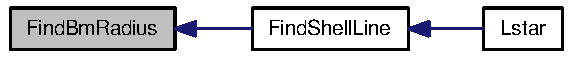
\includegraphics[width=155pt]{_lgm___lstar_info_8h_15d887d6b99cb83ce58b5a04a171ec67_icgraph}
\end{center}
\end{figure}
\hypertarget{_lgm___lstar_info_8h_e79603e88bcb7860ca33e8fe4fbdf37f}{
\index{Lgm\_\-LstarInfo.h@{Lgm\_\-LstarInfo.h}!FindShellLine@{FindShellLine}}
\index{FindShellLine@{FindShellLine}!Lgm_LstarInfo.h@{Lgm\_\-LstarInfo.h}}
\subsubsection[{FindShellLine}]{\setlength{\rightskip}{0pt plus 5cm}int FindShellLine (double {\em I0}, \/  double $\ast$ {\em Ifound}, \/  double {\em Bm}, \/  double {\em MLT}, \/  double $\ast$ {\em mlat}, \/  double $\ast$ {\em rad}, \/  double {\em mlat0}, \/  double {\em mlat1}, \/  {\bf Lgm\_\-LstarInfo} $\ast$ {\em LstarInfo})}}
\label{_lgm___lstar_info_8h_e79603e88bcb7860ca33e8fe4fbdf37f}




Definition at line 36 of file DriftShell.c.

Here is the call graph for this function:\nopagebreak
\begin{figure}[H]
\begin{center}
\leavevmode
\includegraphics[width=401pt]{_lgm___lstar_info_8h_e79603e88bcb7860ca33e8fe4fbdf37f_cgraph}
\end{center}
\end{figure}


Here is the caller graph for this function:\nopagebreak
\begin{figure}[H]
\begin{center}
\leavevmode
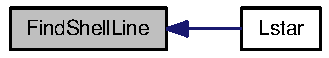
\includegraphics[width=97pt]{_lgm___lstar_info_8h_e79603e88bcb7860ca33e8fe4fbdf37f_icgraph}
\end{center}
\end{figure}
\hypertarget{_lgm___lstar_info_8h_e2e73ba3832c389e53954019ceb47ded}{
\index{Lgm\_\-LstarInfo.h@{Lgm\_\-LstarInfo.h}!spline@{spline}}
\index{spline@{spline}!Lgm_LstarInfo.h@{Lgm\_\-LstarInfo.h}}
\subsubsection[{spline}]{\setlength{\rightskip}{0pt plus 5cm}void spline (double $\ast$ {\em x}, \/  double $\ast$ {\em y}, \/  int {\em n}, \/  double {\em yp1}, \/  double {\em ypn}, \/  double $\ast$ {\em y2})}}
\label{_lgm___lstar_info_8h_e2e73ba3832c389e53954019ceb47ded}




Here is the caller graph for this function:\nopagebreak
\begin{figure}[H]
\begin{center}
\leavevmode
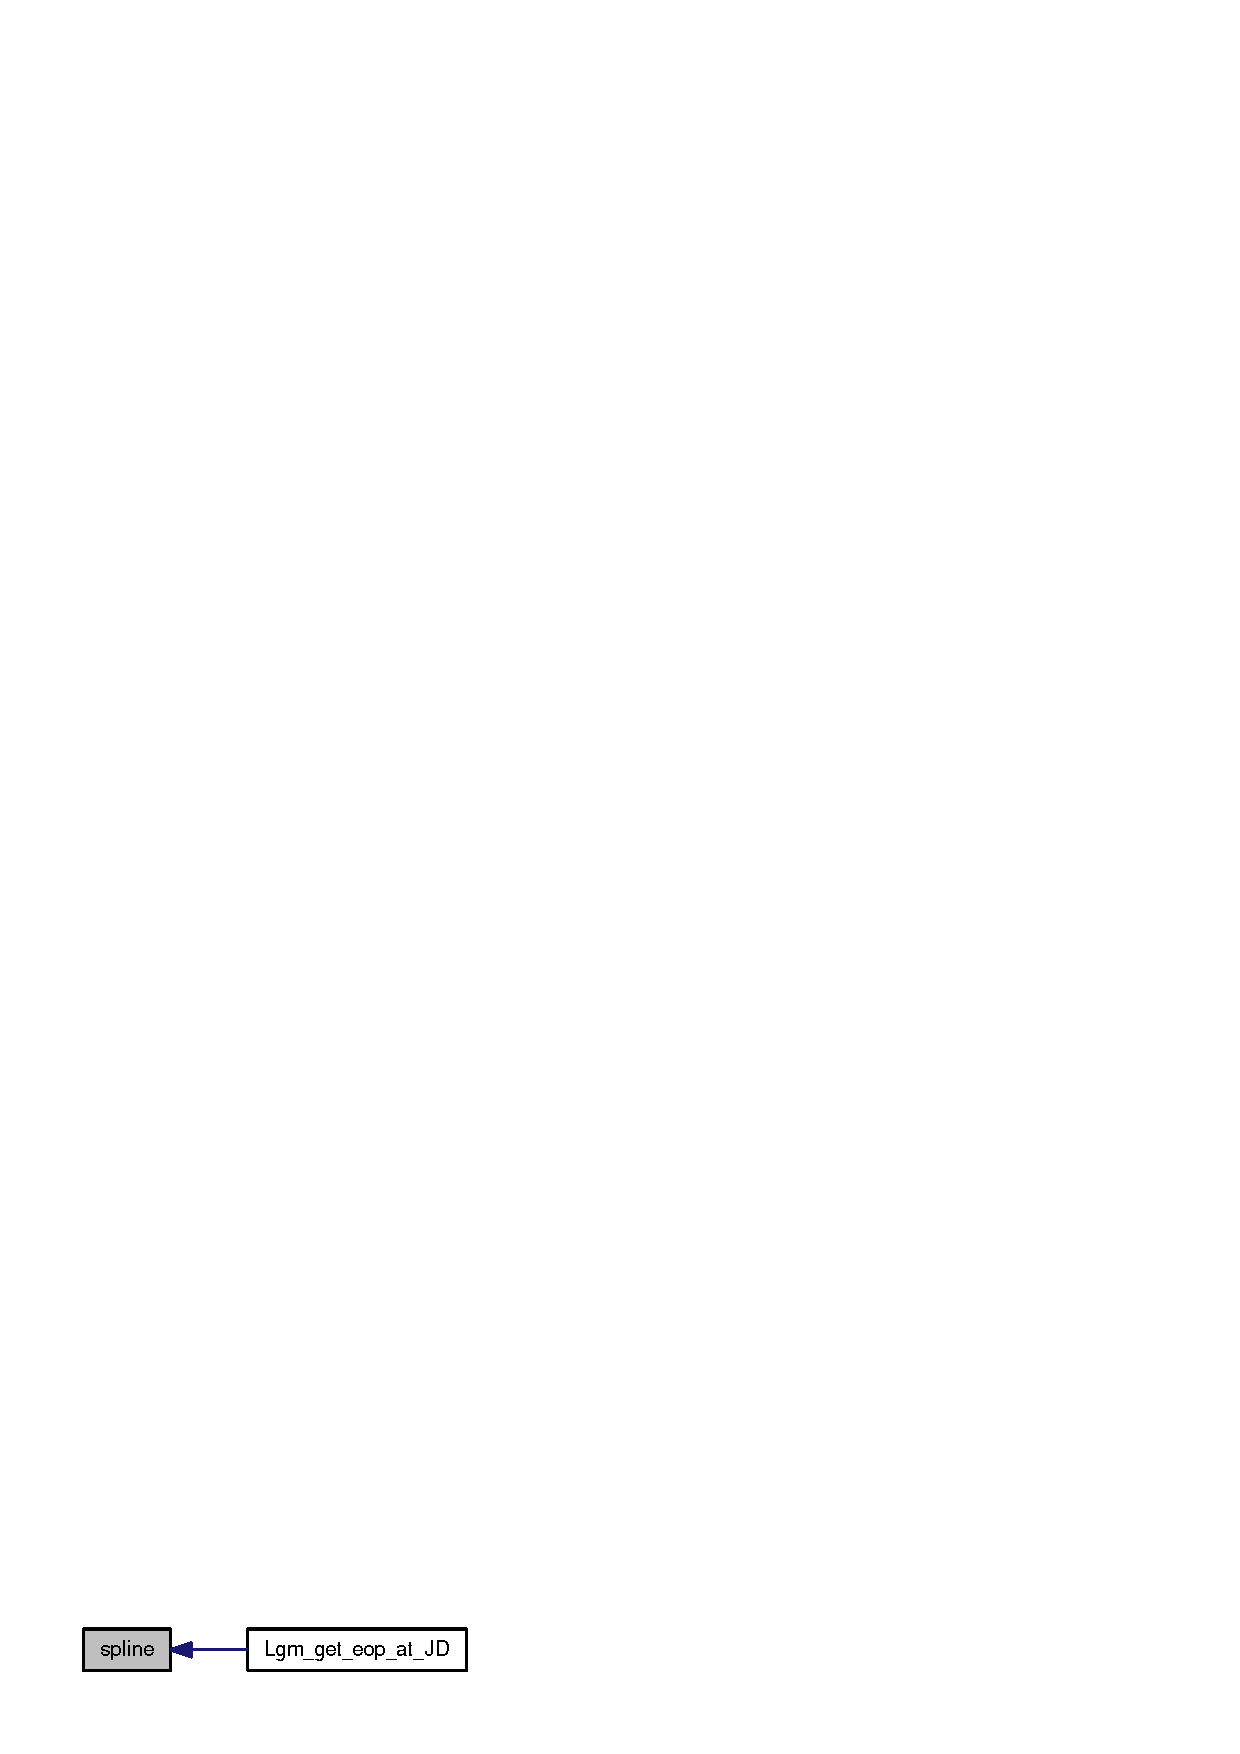
\includegraphics[width=114pt]{_lgm___lstar_info_8h_e2e73ba3832c389e53954019ceb47ded_icgraph}
\end{center}
\end{figure}
\hypertarget{_lgm___lstar_info_8h_219484a4d3318d5361a52365d97cddc3}{
\index{Lgm\_\-LstarInfo.h@{Lgm\_\-LstarInfo.h}!splint@{splint}}
\index{splint@{splint}!Lgm_LstarInfo.h@{Lgm\_\-LstarInfo.h}}
\subsubsection[{splint}]{\setlength{\rightskip}{0pt plus 5cm}void splint (double $\ast$ {\em xa}, \/  double $\ast$ {\em ya}, \/  double $\ast$ {\em y2a}, \/  int {\em n}, \/  double {\em x}, \/  double $\ast$ {\em y})}}
\label{_lgm___lstar_info_8h_219484a4d3318d5361a52365d97cddc3}


\hypertarget{_lgm___lstar_info_8h_e2628883d2b8f49b8df3690a121f1e40}{
\index{Lgm\_\-LstarInfo.h@{Lgm\_\-LstarInfo.h}!quicksort@{quicksort}}
\index{quicksort@{quicksort}!Lgm_LstarInfo.h@{Lgm\_\-LstarInfo.h}}
\subsubsection[{quicksort}]{\setlength{\rightskip}{0pt plus 5cm}void quicksort (unsigned long {\em n}, \/  double $\ast$ {\em arr})}}
\label{_lgm___lstar_info_8h_e2628883d2b8f49b8df3690a121f1e40}




Definition at line 7 of file quicksort.c.\hypertarget{_lgm___lstar_info_8h_3801a78bfafe0c674baf406ff2531f3e}{
\index{Lgm\_\-LstarInfo.h@{Lgm\_\-LstarInfo.h}!quicksort2@{quicksort2}}
\index{quicksort2@{quicksort2}!Lgm_LstarInfo.h@{Lgm\_\-LstarInfo.h}}
\subsubsection[{quicksort2}]{\setlength{\rightskip}{0pt plus 5cm}void quicksort2 (unsigned long {\em n}, \/  double $\ast$ {\em arr}, \/  double $\ast$ {\em brr})}}
\label{_lgm___lstar_info_8h_3801a78bfafe0c674baf406ff2531f3e}




Definition at line 74 of file quicksort.c.

Here is the caller graph for this function:\nopagebreak
\begin{figure}[H]
\begin{center}
\leavevmode
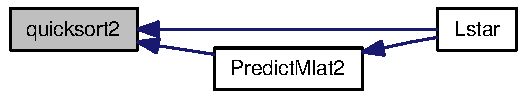
\includegraphics[width=144pt]{_lgm___lstar_info_8h_3801a78bfafe0c674baf406ff2531f3e_icgraph}
\end{center}
\end{figure}
\hypertarget{_lgm___lstar_info_8h_0d0473dc2b48c646fb6cf5297ba74636}{
\index{Lgm\_\-LstarInfo.h@{Lgm\_\-LstarInfo.h}!init\_\-info@{init\_\-info}}
\index{init\_\-info@{init\_\-info}!Lgm_LstarInfo.h@{Lgm\_\-LstarInfo.h}}
\subsubsection[{init\_\-info}]{\setlength{\rightskip}{0pt plus 5cm}{\bf Lgm\_\-MagModelInfo}$\ast$ init\_\-info ()}}
\label{_lgm___lstar_info_8h_0d0473dc2b48c646fb6cf5297ba74636}


\hypertarget{_lgm___lstar_info_8h_68ec464c1b33f0b437d856629f0dd901}{
\index{Lgm\_\-LstarInfo.h@{Lgm\_\-LstarInfo.h}!NewTimeLstarInfo@{NewTimeLstarInfo}}
\index{NewTimeLstarInfo@{NewTimeLstarInfo}!Lgm_LstarInfo.h@{Lgm\_\-LstarInfo.h}}
\subsubsection[{NewTimeLstarInfo}]{\setlength{\rightskip}{0pt plus 5cm}void NewTimeLstarInfo (long int {\em Date}, \/  double {\em UT}, \/  double {\em PitchAngle}, \/  int($\ast$)({\bf Lgm\_\-Vector} $\ast$, {\bf Lgm\_\-Vector} $\ast$, {\bf Lgm\_\-MagModelInfo} $\ast$) {\em Mag}, \/  {\bf Lgm\_\-LstarInfo} $\ast$ {\em LstarInfo})}}
\label{_lgm___lstar_info_8h_68ec464c1b33f0b437d856629f0dd901}




Definition at line 281 of file ComputeLstar.c.

Here is the call graph for this function:\nopagebreak
\begin{figure}[H]
\begin{center}
\leavevmode
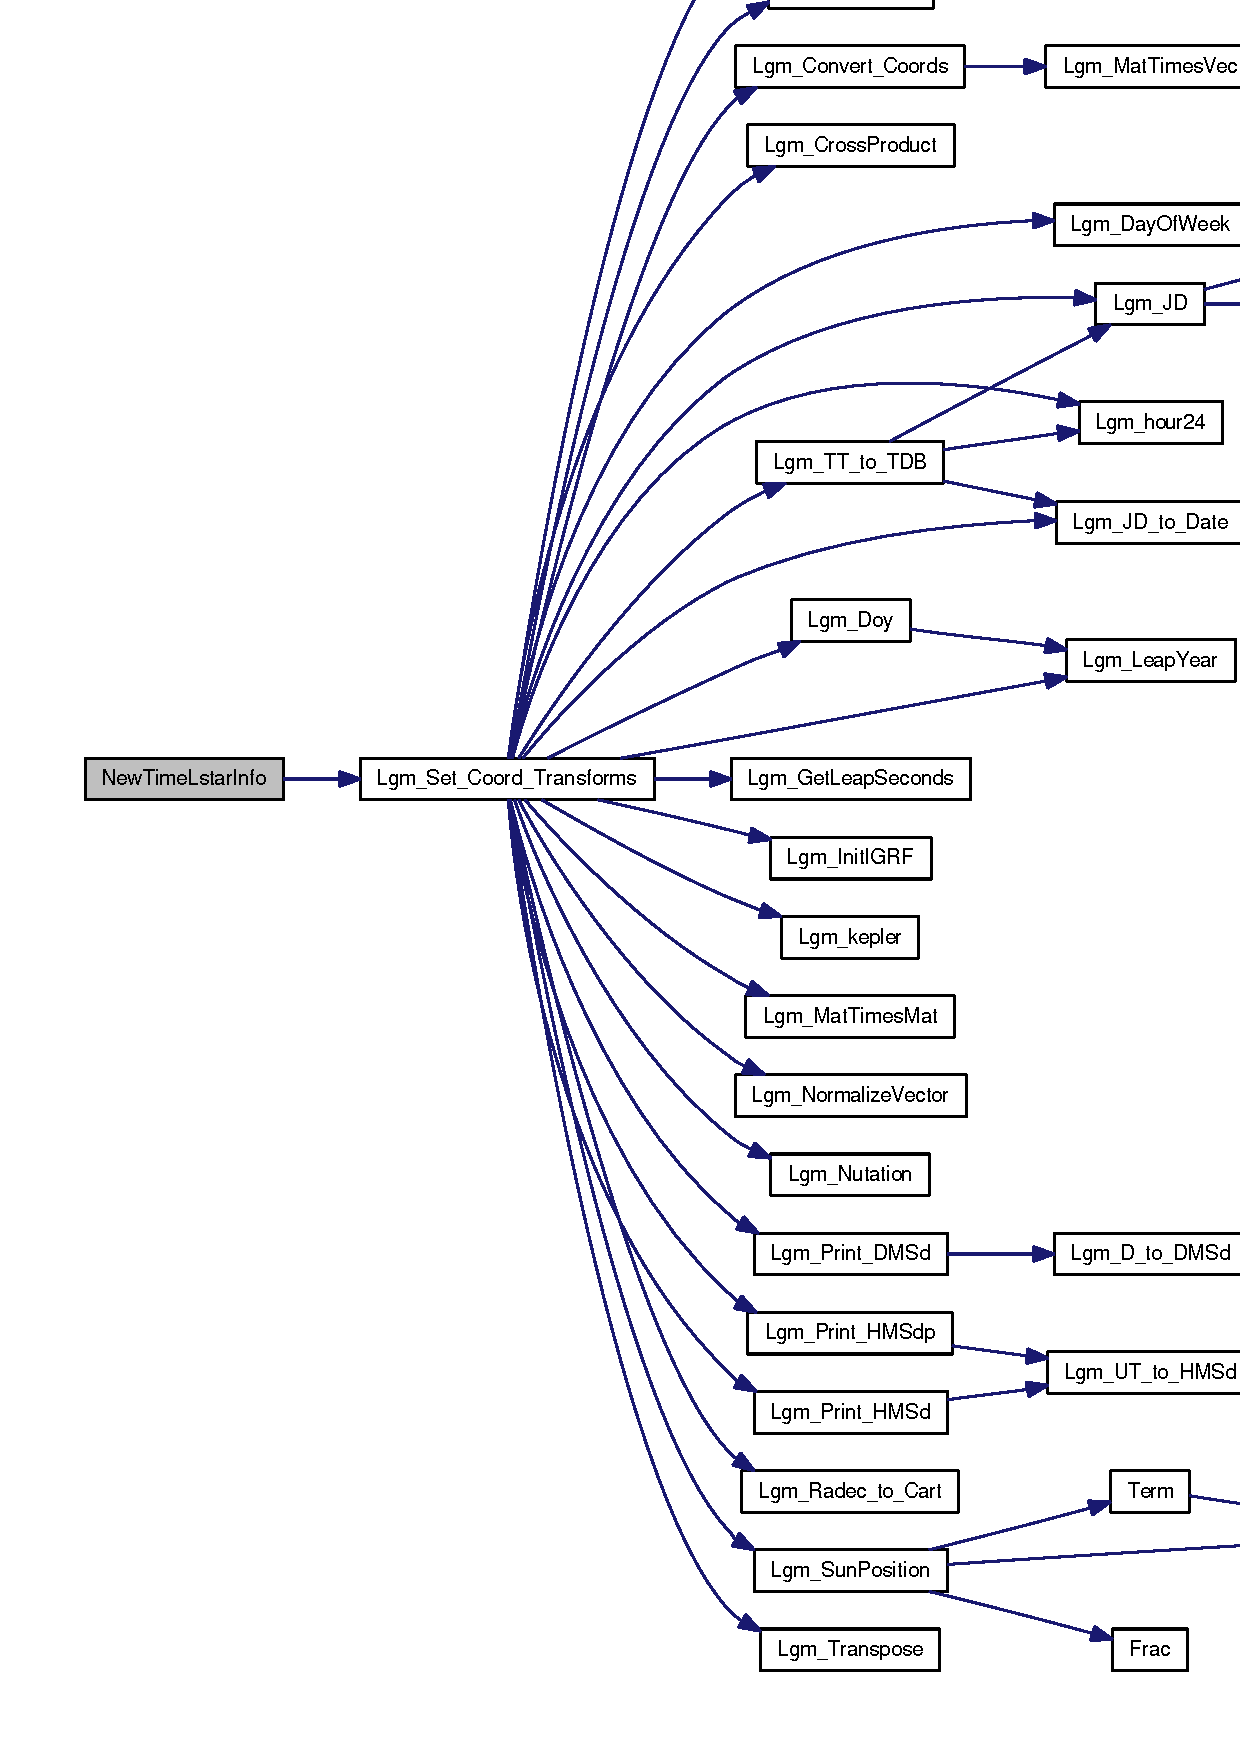
\includegraphics[width=381pt]{_lgm___lstar_info_8h_68ec464c1b33f0b437d856629f0dd901_cgraph}
\end{center}
\end{figure}
\hypertarget{_lgm___lstar_info_8h_957a4d60eb4025656b3c2557b402523e}{
\index{Lgm\_\-LstarInfo.h@{Lgm\_\-LstarInfo.h}!Lstar@{Lstar}}
\index{Lstar@{Lstar}!Lgm_LstarInfo.h@{Lgm\_\-LstarInfo.h}}
\subsubsection[{Lstar}]{\setlength{\rightskip}{0pt plus 5cm}int Lstar ({\bf Lgm\_\-Vector} $\ast$ {\em vin}, \/  {\bf Lgm\_\-LstarInfo} $\ast$ {\em LstarInfo})}}
\label{_lgm___lstar_info_8h_957a4d60eb4025656b3c2557b402523e}




Definition at line 307 of file ComputeLstar.c.

Here is the call graph for this function:\nopagebreak
\begin{figure}[H]
\begin{center}
\leavevmode
\includegraphics[width=420pt]{_lgm___lstar_info_8h_957a4d60eb4025656b3c2557b402523e_cgraph}
\end{center}
\end{figure}
\hypertarget{_lgm___lstar_info_8h_871565dbd20b1df061fb2e706bd724db}{
\index{Lgm\_\-LstarInfo.h@{Lgm\_\-LstarInfo.h}!MagFlux@{MagFlux}}
\index{MagFlux@{MagFlux}!Lgm_LstarInfo.h@{Lgm\_\-LstarInfo.h}}
\subsubsection[{MagFlux}]{\setlength{\rightskip}{0pt plus 5cm}double MagFlux ({\bf Lgm\_\-LstarInfo} $\ast$ {\em LstarInfo})}}
\label{_lgm___lstar_info_8h_871565dbd20b1df061fb2e706bd724db}




Definition at line 842 of file ComputeLstar.c.

Here is the call graph for this function:\nopagebreak
\begin{figure}[H]
\begin{center}
\leavevmode
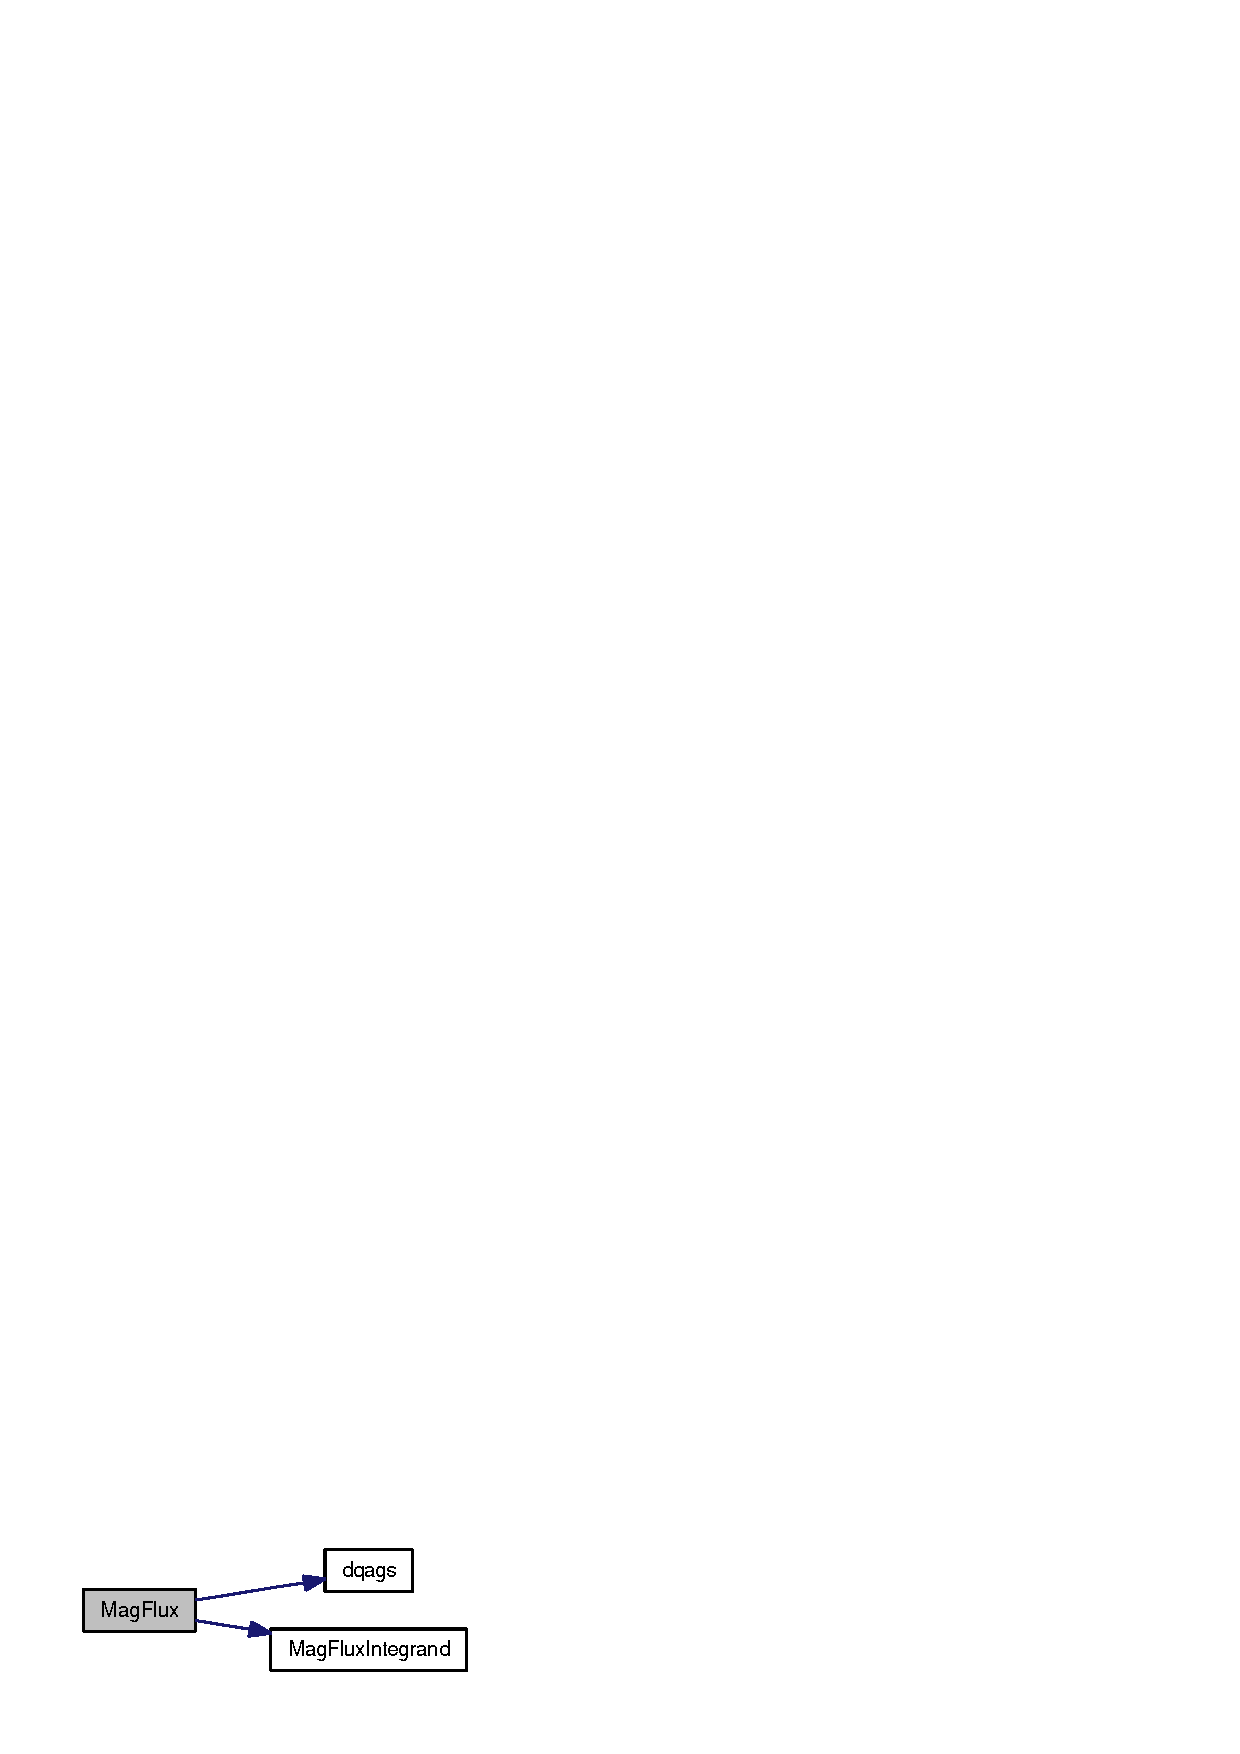
\includegraphics[width=114pt]{_lgm___lstar_info_8h_871565dbd20b1df061fb2e706bd724db_cgraph}
\end{center}
\end{figure}


Here is the caller graph for this function:\nopagebreak
\begin{figure}[H]
\begin{center}
\leavevmode
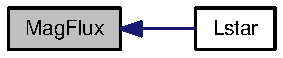
\includegraphics[width=86pt]{_lgm___lstar_info_8h_871565dbd20b1df061fb2e706bd724db_icgraph}
\end{center}
\end{figure}
\hypertarget{_lgm___lstar_info_8h_7da6f58b128b4aef809400ada95767d4}{
\index{Lgm\_\-LstarInfo.h@{Lgm\_\-LstarInfo.h}!MagFlux2@{MagFlux2}}
\index{MagFlux2@{MagFlux2}!Lgm_LstarInfo.h@{Lgm\_\-LstarInfo.h}}
\subsubsection[{MagFlux2}]{\setlength{\rightskip}{0pt plus 5cm}double MagFlux2 ({\bf Lgm\_\-LstarInfo} $\ast$ {\em LstarInfo})}}
\label{_lgm___lstar_info_8h_7da6f58b128b4aef809400ada95767d4}




Definition at line 1023 of file ComputeLstar.c.

Here is the call graph for this function:\nopagebreak
\begin{figure}[H]
\begin{center}
\leavevmode
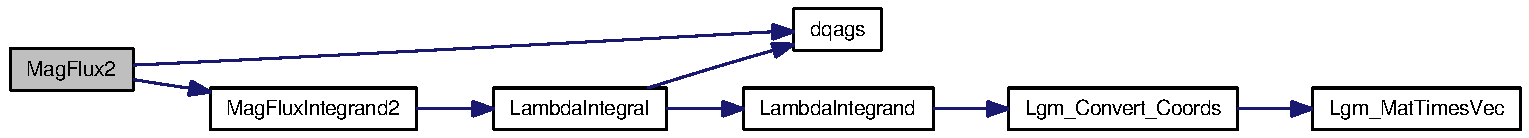
\includegraphics[width=385pt]{_lgm___lstar_info_8h_7da6f58b128b4aef809400ada95767d4_cgraph}
\end{center}
\end{figure}


Here is the caller graph for this function:\nopagebreak
\begin{figure}[H]
\begin{center}
\leavevmode
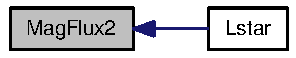
\includegraphics[width=89pt]{_lgm___lstar_info_8h_7da6f58b128b4aef809400ada95767d4_icgraph}
\end{center}
\end{figure}
\hypertarget{_lgm___lstar_info_8h_5f75b0909329fb6260c63bc551c29acb}{
\index{Lgm\_\-LstarInfo.h@{Lgm\_\-LstarInfo.h}!MagFluxIntegrand@{MagFluxIntegrand}}
\index{MagFluxIntegrand@{MagFluxIntegrand}!Lgm_LstarInfo.h@{Lgm\_\-LstarInfo.h}}
\subsubsection[{MagFluxIntegrand}]{\setlength{\rightskip}{0pt plus 5cm}double MagFluxIntegrand (double {\em Phi}, \/  {\bf \_\-qpInfo} $\ast$ {\em qpInfo})}}
\label{_lgm___lstar_info_8h_5f75b0909329fb6260c63bc551c29acb}




Definition at line 815 of file ComputeLstar.c.

Here is the caller graph for this function:\nopagebreak
\begin{figure}[H]
\begin{center}
\leavevmode
\includegraphics[width=151pt]{_lgm___lstar_info_8h_5f75b0909329fb6260c63bc551c29acb_icgraph}
\end{center}
\end{figure}
\hypertarget{_lgm___lstar_info_8h_0f767b7206b1928b2f36fa7c5a26ca33}{
\index{Lgm\_\-LstarInfo.h@{Lgm\_\-LstarInfo.h}!MagFluxIntegrand2@{MagFluxIntegrand2}}
\index{MagFluxIntegrand2@{MagFluxIntegrand2}!Lgm_LstarInfo.h@{Lgm\_\-LstarInfo.h}}
\subsubsection[{MagFluxIntegrand2}]{\setlength{\rightskip}{0pt plus 5cm}double MagFluxIntegrand2 (double {\em Phi}, \/  {\bf \_\-qpInfo} $\ast$ {\em qpInfo})}}
\label{_lgm___lstar_info_8h_0f767b7206b1928b2f36fa7c5a26ca33}




Definition at line 1005 of file ComputeLstar.c.

Here is the call graph for this function:\nopagebreak
\begin{figure}[H]
\begin{center}
\leavevmode
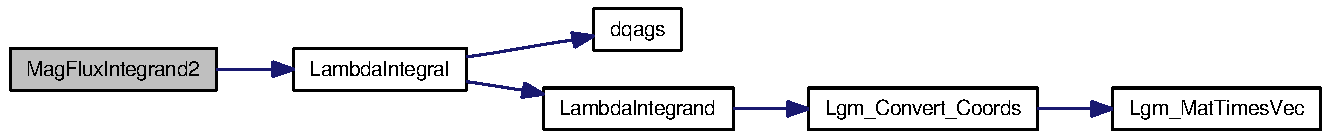
\includegraphics[width=337pt]{_lgm___lstar_info_8h_0f767b7206b1928b2f36fa7c5a26ca33_cgraph}
\end{center}
\end{figure}


Here is the caller graph for this function:\nopagebreak
\begin{figure}[H]
\begin{center}
\leavevmode
\includegraphics[width=157pt]{_lgm___lstar_info_8h_0f767b7206b1928b2f36fa7c5a26ca33_icgraph}
\end{center}
\end{figure}
\hypertarget{_lgm___lstar_info_8h_fb4cfc3e9728d5ec4867d39f1384dc38}{
\index{Lgm\_\-LstarInfo.h@{Lgm\_\-LstarInfo.h}!LambdaIntegrand@{LambdaIntegrand}}
\index{LambdaIntegrand@{LambdaIntegrand}!Lgm_LstarInfo.h@{Lgm\_\-LstarInfo.h}}
\subsubsection[{LambdaIntegrand}]{\setlength{\rightskip}{0pt plus 5cm}double LambdaIntegrand (double {\em Lambda}, \/  {\bf \_\-qpInfo} $\ast$ {\em qpInfo})}}
\label{_lgm___lstar_info_8h_fb4cfc3e9728d5ec4867d39f1384dc38}




Definition at line 909 of file ComputeLstar.c.

Here is the call graph for this function:\nopagebreak
\begin{figure}[H]
\begin{center}
\leavevmode
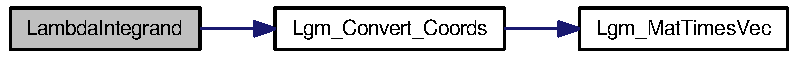
\includegraphics[width=209pt]{_lgm___lstar_info_8h_fb4cfc3e9728d5ec4867d39f1384dc38_cgraph}
\end{center}
\end{figure}


Here is the caller graph for this function:\nopagebreak
\begin{figure}[H]
\begin{center}
\leavevmode
\includegraphics[width=281pt]{_lgm___lstar_info_8h_fb4cfc3e9728d5ec4867d39f1384dc38_icgraph}
\end{center}
\end{figure}
\hypertarget{_lgm___lstar_info_8h_593bd0ac5cd8b137cbc401b58219df31}{
\index{Lgm\_\-LstarInfo.h@{Lgm\_\-LstarInfo.h}!LambdaIntegral@{LambdaIntegral}}
\index{LambdaIntegral@{LambdaIntegral}!Lgm_LstarInfo.h@{Lgm\_\-LstarInfo.h}}
\subsubsection[{LambdaIntegral}]{\setlength{\rightskip}{0pt plus 5cm}double LambdaIntegral ({\bf Lgm\_\-LstarInfo} $\ast$ {\em LstarInfo})}}
\label{_lgm___lstar_info_8h_593bd0ac5cd8b137cbc401b58219df31}




Definition at line 945 of file ComputeLstar.c.

Here is the call graph for this function:\nopagebreak
\begin{figure}[H]
\begin{center}
\leavevmode
\includegraphics[width=269pt]{_lgm___lstar_info_8h_593bd0ac5cd8b137cbc401b58219df31_cgraph}
\end{center}
\end{figure}


Here is the caller graph for this function:\nopagebreak
\begin{figure}[H]
\begin{center}
\leavevmode
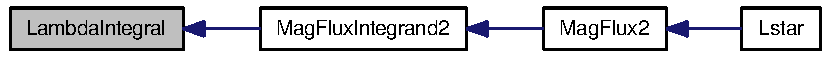
\includegraphics[width=217pt]{_lgm___lstar_info_8h_593bd0ac5cd8b137cbc401b58219df31_icgraph}
\end{center}
\end{figure}
\hypertarget{_lgm___lstar_info_8h_48c5ace9102643dda45f657ddb8aac3c}{
\index{Lgm\_\-LstarInfo.h@{Lgm\_\-LstarInfo.h}!AngVelInv@{AngVelInv}}
\index{AngVelInv@{AngVelInv}!Lgm_LstarInfo.h@{Lgm\_\-LstarInfo.h}}
\subsubsection[{AngVelInv}]{\setlength{\rightskip}{0pt plus 5cm}double AngVelInv (double {\em Phi})}}
\label{_lgm___lstar_info_8h_48c5ace9102643dda45f657ddb8aac3c}


